% !TEX root = ../main.tex
%==============================================================
\chapter{Đánh giá}
\label{ch:danh-gia}

Chương này trình bày kết quả thực nghiệm của hệ thống đã hiện thực ở
Chương~\ref{ch:trien-khai}. Phần đầu mô tả cấu hình phần cứng và phần mềm dùng
để thử nghiệm. Phần sau phân tích các ảnh kết xuất theo từng nhóm hiệu ứng:
chất lượng tổng thể, tái tạo vật liệu, độ sâu trường ảnh, nhòe chuyển động và làm
tối rìa ảnh, kèm theo số liệu hiệu năng đo trực tiếp trong quá trình kết xuất.

\section{Môi trường thử nghiệm}
Toàn bộ thử nghiệm được thực hiện trên một máy tính xách tay với cấu hình nêu ở
Bảng~\ref{tab:moi-truong}. Card đồ họa thuộc phân khúc phổ thông, dung lượng bộ
nhớ video giới hạn ở 4\,GB, nên kết quả hiệu năng phản ánh mức trung bình thấp
của phần cứng người dùng phổ thông.

\begin{table}[H]
  \centering
  \caption{Cấu hình môi trường thử nghiệm.}
  \label{tab:moi-truong}
  \begin{tabularx}{\textwidth}{l X}
    \toprule
    \textbf{Thành phần} & \textbf{Thông số} \\
    \midrule
    CPU              & AMD Ryzen 5 5600H, 6 nhân 12 luồng \\
    GPU              & NVIDIA GeForce GTX 1650, 4\,GB GDDR \\
    Bộ nhớ hệ thống  & 16\,GB \\
    Hệ điều hành     & Windows 11, 64-bit \\
    CUDA Toolkit     & phiên bản 12.6 \\
    Trình biên dịch  & MSVC kết hợp \texttt{nvcc} \\
    Độ phân giải kết xuất & 1920 $\times$ 1014 điểm ảnh \\
    \bottomrule
  \end{tabularx}
\end{table}

Hiệu năng được đo bằng hai chỉ số hiển thị trực tiếp trên bảng điều khiển: thời
gian kết xuất trung bình của một khung hình tính bằng mili giây và số khung hình
trên giây tương ứng. Mỗi khung hình lấy một mẫu cho mỗi điểm ảnh, sau đó cộng dồn
vào bộ đệm tích lũy nên ảnh hội tụ dần theo thời gian. Số khung hình tích lũy
được ghi nhận để thể hiện mức độ hội tụ của ảnh tại thời điểm chụp.

\section{Chất lượng kết xuất tổng thể}
Hình~\ref{fig:best-render} là ảnh kết xuất trên cảnh có mật độ vật thể cao gồm
vài trăm khối cầu với đủ ba loại vật liệu. Nguyên lý cốt lõi quyết định chất
lượng ảnh ở đây là tích lũy Monte Carlo theo thời gian: mỗi khung chỉ lấy một mẫu
ngẫu nhiên cho mỗi điểm ảnh nên rất nhiễu, nhưng khi lấy trung bình $N$ mẫu độc
lập qua các khung liên tiếp, phương sai của bộ ước lượng \eqref{eq:montecarlo}
giảm theo $1/N$ và biên độ nhiễu (độ lệch chuẩn) giảm theo $1/\sqrt{N}$. Chính
quy luật $O(1/\sqrt{N})$ này giải thích vì sao ảnh hội tụ nhanh lúc đầu rồi chậm
dần: sau 1846 khung hình tích lũy, nhiễu hạt gần như bị khử hoàn toàn và các hiệu
ứng phản xạ, khúc xạ, đổ bóng mềm được tái tạo nhất quán. Muốn giảm tiếp một nửa
nhiễu còn lại cần gấp bốn lần số khung, đúng như hệ quả của quy luật này.
Ở cảnh đông đối tượng như vậy, thời gian mỗi khung tăng lên khoảng 542\,ms tương
ứng 1{,}8 khung hình trên giây, do mỗi tia phải duyệt tuyến tính qua toàn bộ
danh sách vật thể để tìm giao điểm. Đây là hệ quả trực tiếp của việc chưa dùng
cấu trúc tăng tốc không gian, và là động lực cho hướng tối ưu bằng BVH nêu ở
Chương~\ref{ch:ket-luan}.

\begin{figure}[H]
  \centering
  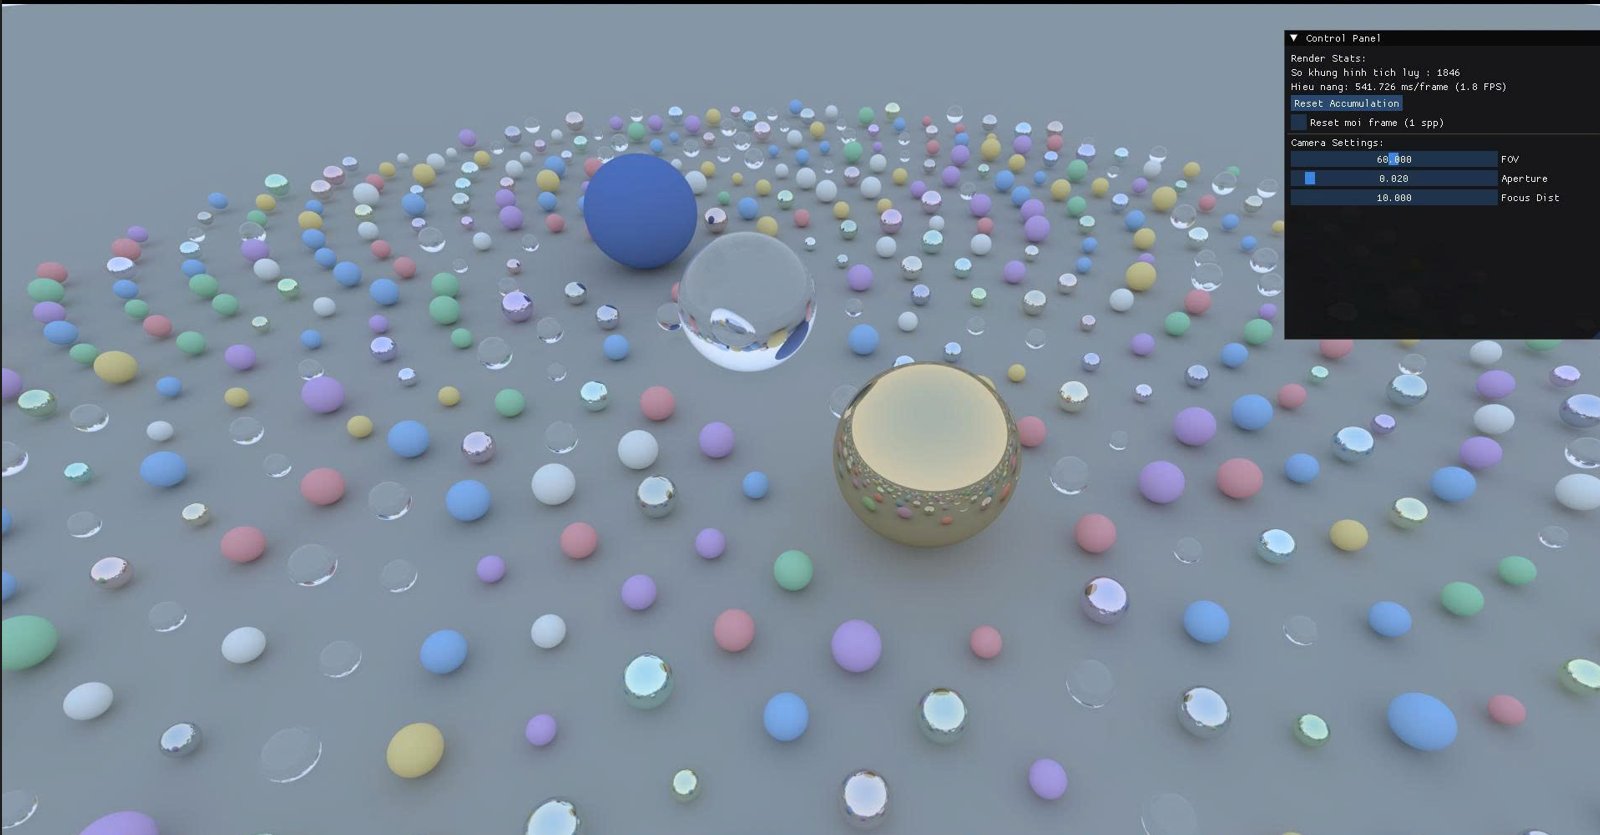
\includegraphics[width=\textwidth]{images/best_render.png}
  \caption{Ảnh kết xuất trên cảnh mật độ cao sau 1846 khung hình tích lũy.}
  \label{fig:best-render}
\end{figure}

\section{Tái tạo các loại vật liệu}
Hình~\ref{fig:three-materials} kiểm chứng riêng ba loại vật liệu đã hiện thực
trên một cảnh thưa để quan sát rõ từng đặc tính, mỗi loại tương ứng một cơ chế
tán xạ khác nhau. Khối cầu màu đỏ là vật liệu Lambertian: bề mặt khuếch tán lý
tưởng có hàm phản xạ hằng số $f_r=\rho/\pi$, tán xạ ánh sáng đều theo mọi hướng
nên bề mặt sáng đục và không phản chiếu môi trường. Khối cầu trong suốt là vật
liệu điện môi: phần khúc xạ tuân theo định luật Snell~\eqref{eq:snell} bẻ cong tia
qua thân cầu làm đảo ngược ảnh nền, còn tỉ lệ năng lượng phản xạ ở rìa tăng vọt
theo xấp xỉ Schlick $R(\theta)=R_0+(1-R_0)(1-\cos\theta)^5$~\eqref{eq:schlick} —
đó là lý do viền cầu sáng và phản chiếu rõ hơn phần giữa. Khối cầu vàng kim là
vật liệu kim loại: tia phản xạ gương quanh pháp tuyến theo
$\mathbf{r}=\mathbf{d}-2(\mathbf{d}\cdot\mathbf{n})\mathbf{n}$~\eqref{eq:reflect}
nên bề mặt ánh lên hình ảnh các vật thể xung quanh. Tại cấu hình khẩu độ bằng 0,
toàn ảnh sắc nét và hệ thống đạt khoảng 57\,ms mỗi khung tương ứng 17{,}5 khung
hình trên giây nhờ số lượng vật thể ít.

\begin{figure}[H]
  \centering
  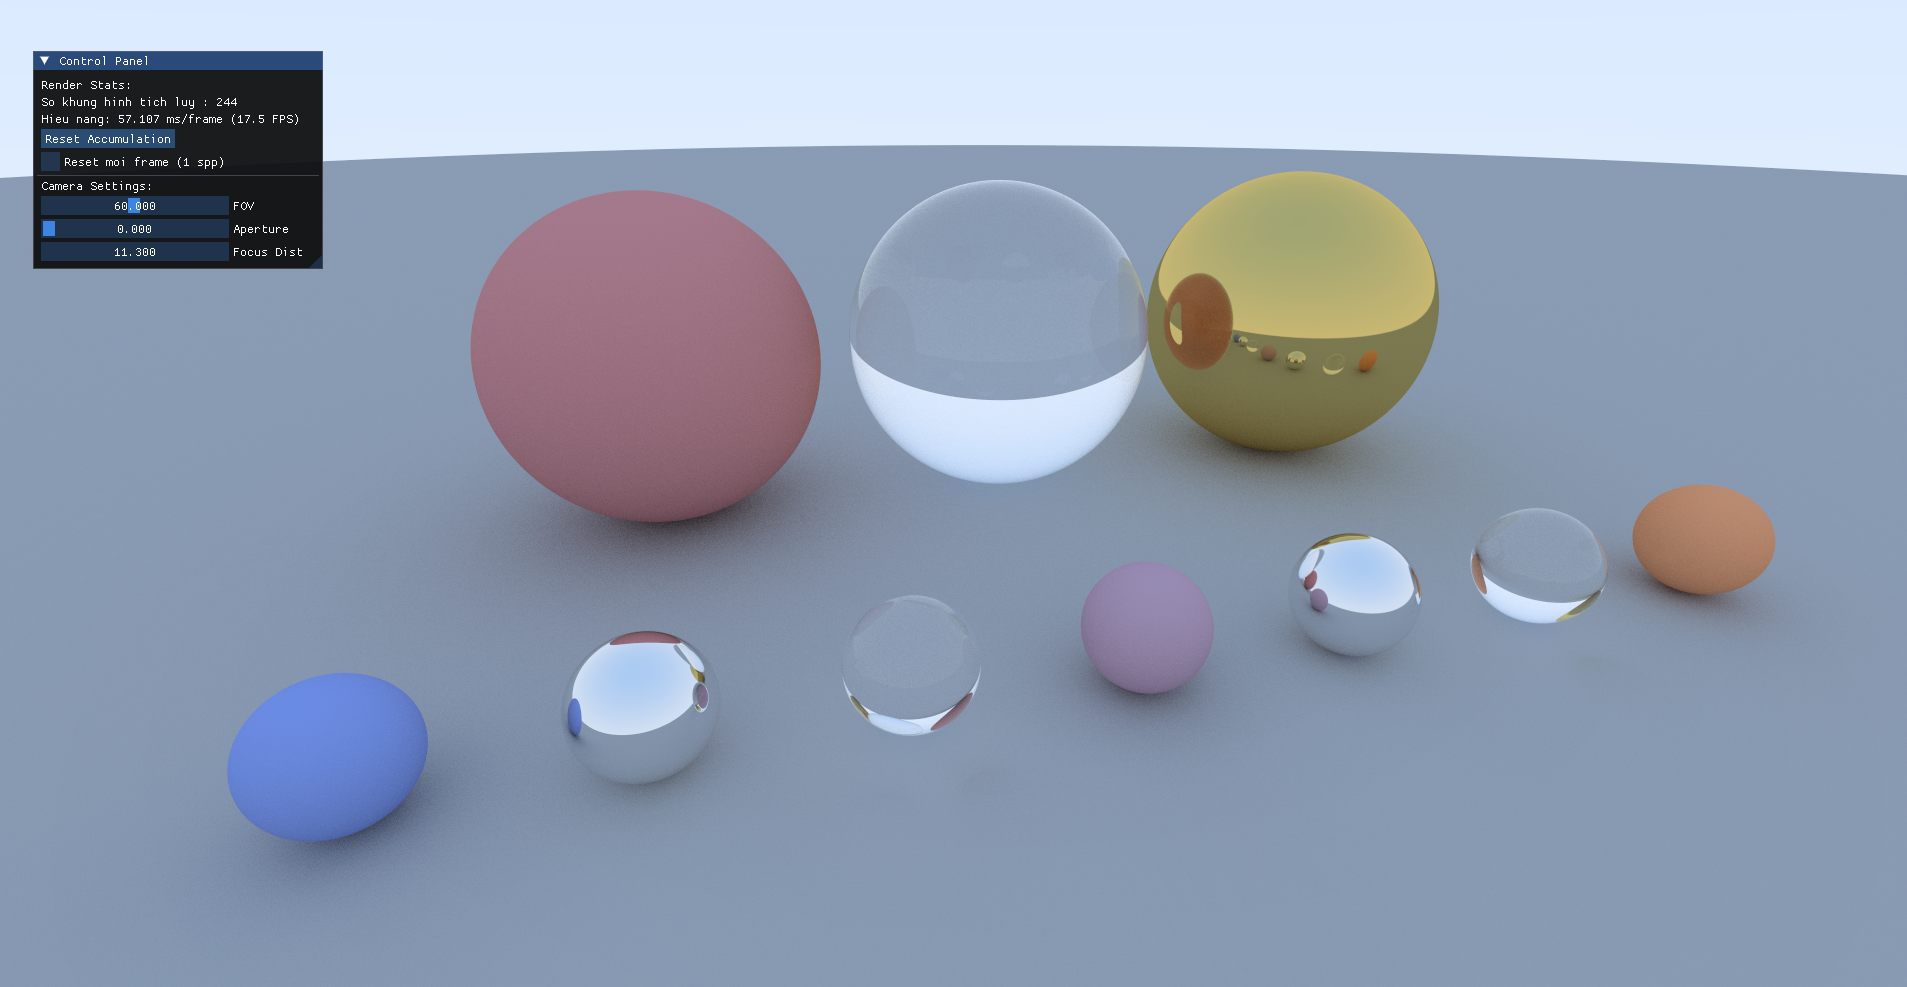
\includegraphics[width=\textwidth]{images/three_materials.png}
  \caption{Ba loại vật liệu Lambertian, điện môi và kim loại trên cùng một cảnh.}
  \label{fig:three-materials}
\end{figure}

\section{Độ sâu trường ảnh}
Hình~\ref{fig:dof} minh họa hai mức khẩu độ khác nhau. Nguyên lý cốt lõi của hiệu
ứng này là khẩu độ hữu hạn của mô hình thấu kính mỏng: mỗi tia không xuất phát từ
một điểm mà từ một vị trí lấy mẫu ngẫu nhiên trên đĩa thấu kính bán kính
$R=\text{khẩu độ}/2$, và mọi tia đều buộc đi qua cùng một điểm trên mặt phẳng lấy
nét. Nhờ vậy vật nằm đúng mặt phẳng lấy nét luôn hội tụ thành một điểm sắc nét;
còn vật ở trước hoặc sau mặt phẳng đó nhận các tia đến từ những vị trí thấu kính
khác nhau nên trải ra thành một đĩa gọi là vòng tròn nhòe. Bán kính vòng nhòe —
và do đó mức độ mờ — tỉ lệ thuận với bán kính khẩu độ $R$: đó là lý do khẩu độ
càng lớn thì vùng rõ nét càng hẹp và hậu cảnh càng mờ. Hiệu ứng phát sinh tự
nhiên từ việc lấy mẫu trên đĩa thấu kính, không cần xử lý hậu kỳ; khi khẩu độ
bằng 0 mô hình thoái biến về camera lỗ kim và toàn ảnh sắc nét.

\begin{figure}[H]
  \centering
  \begin{subfigure}{0.49\textwidth}
    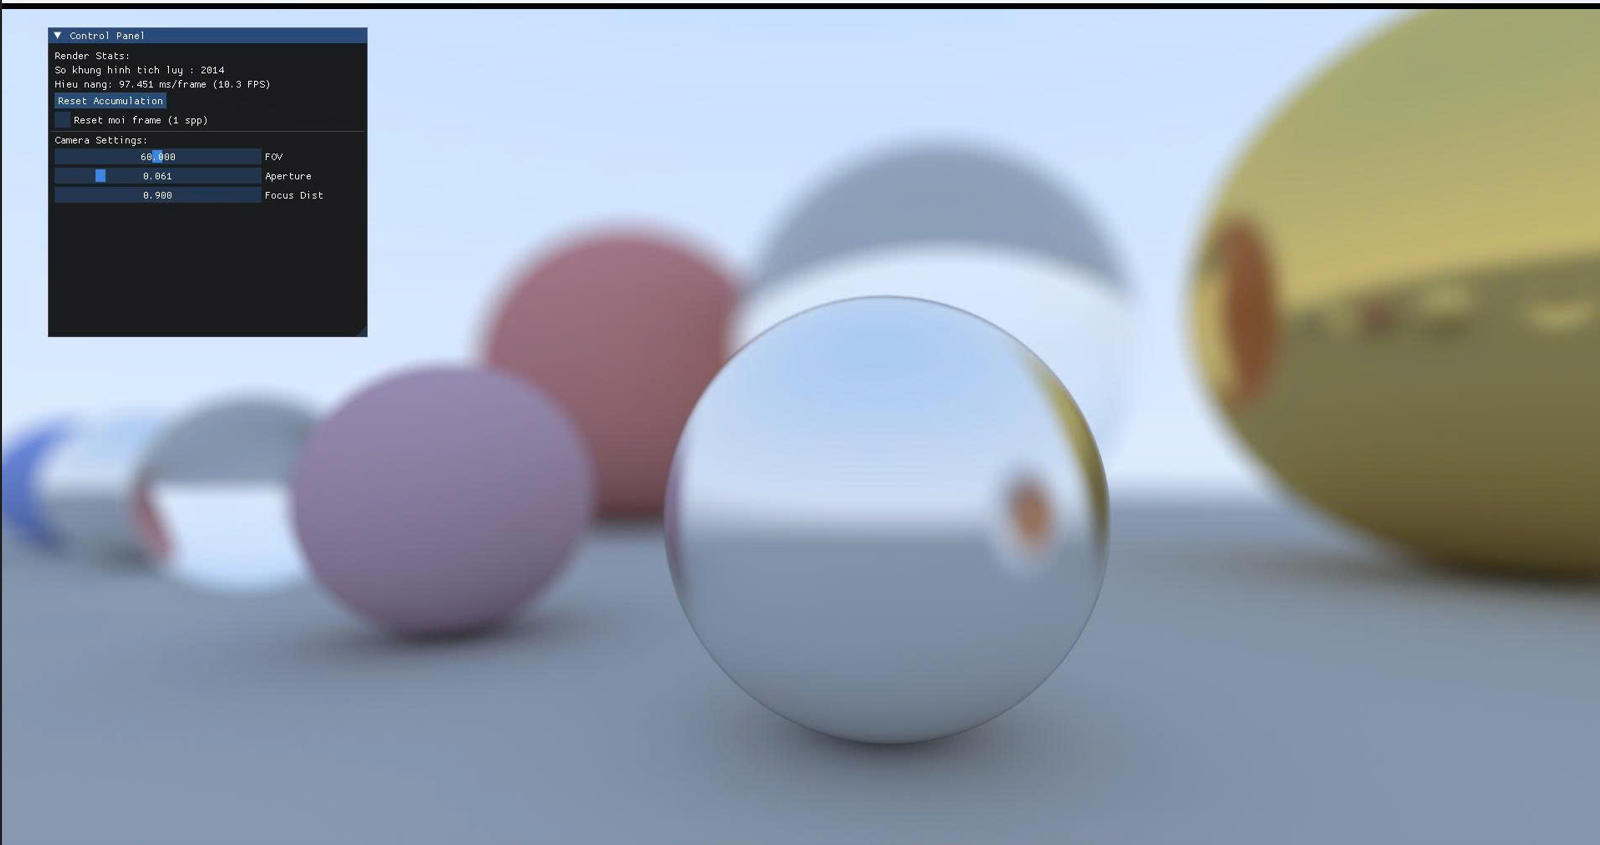
\includegraphics[width=\textwidth]{images/dof_01.png}
    \caption{Khẩu độ 0{,}061, khoảng lấy nét 0{,}9.}
  \end{subfigure}
  \hfill
  \begin{subfigure}{0.49\textwidth}
    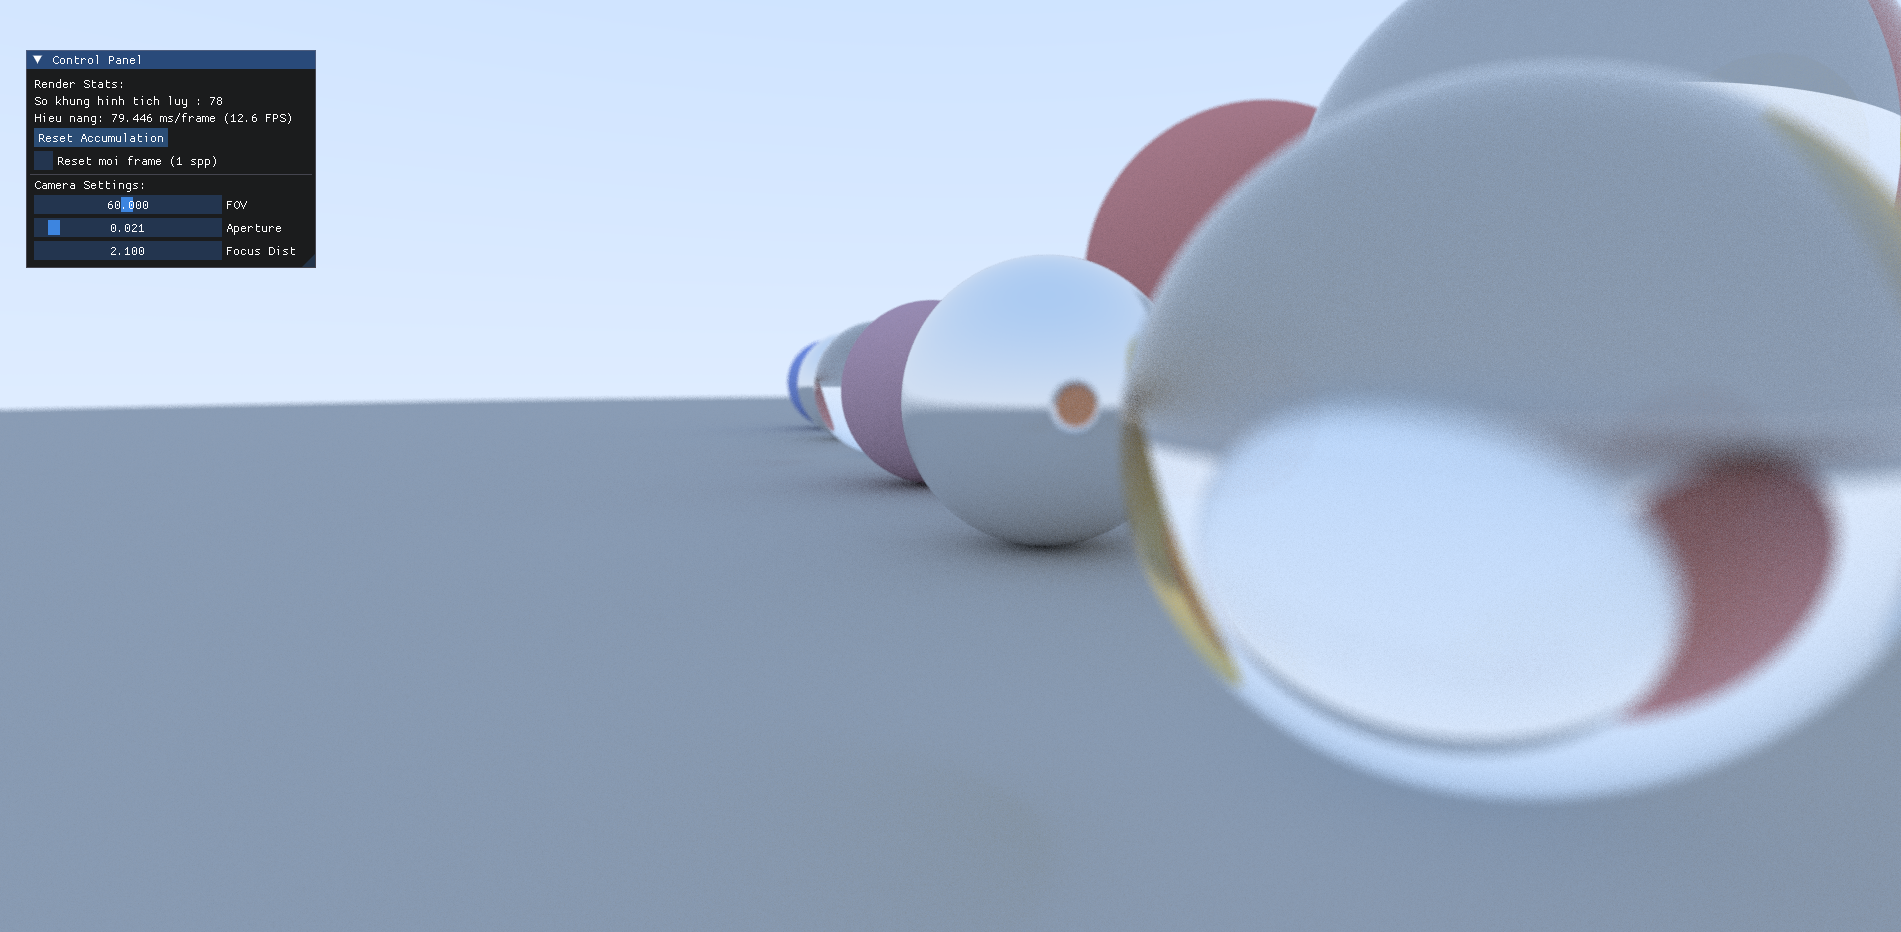
\includegraphics[width=\textwidth]{images/dof_02.png}
    \caption{Khẩu độ 0{,}021, khoảng lấy nét 2{,}1.}
  \end{subfigure}
  \caption{Hiệu ứng độ sâu trường ảnh ở hai cấu hình khẩu độ và khoảng lấy nét.}
  \label{fig:dof}
\end{figure}

\section{Nhòe chuyển động}
Hình~\ref{fig:motion-blur} kiểm chứng hiệu ứng nhòe chuyển động trên cảnh có một
số khối cầu di chuyển. Nguyên lý cốt lõi là camera phơi sáng trong một khoảng
thời gian hữu hạn: giá trị một điểm ảnh không phải bức xạ tại một thời điểm mà là
tích phân của bức xạ theo suốt thời gian màn trập mở $[t_0,t_1]$. Hệ thống ước
lượng tích phân thời gian này bằng Monte Carlo — mỗi tia mang một mốc thời gian
ngẫu nhiên $t\in[t_0,t_1]$, và vị trí khối cầu chuyển động được nội suy tuyến tính
$\mathbf{p}(t)=\mathbf{p}_0+t\,\mathbf{v}$ theo đúng mốc đó. Vì trong một lần phơi
sáng vật đã dịch qua cả quãng đường, năng lượng của nó trải đều dọc quỹ đạo thay
vì đọng tại một chỗ, tạo thành vệt nhòe liên tục; màn trập mở càng lâu (khoảng
$t_1-t_0$ càng lớn) thì vệt nhòe càng dài. Các khối cầu tĩnh không đổi vị trí
theo $t$ nên vẫn sắc nét.

\begin{figure}[H]
  \centering
  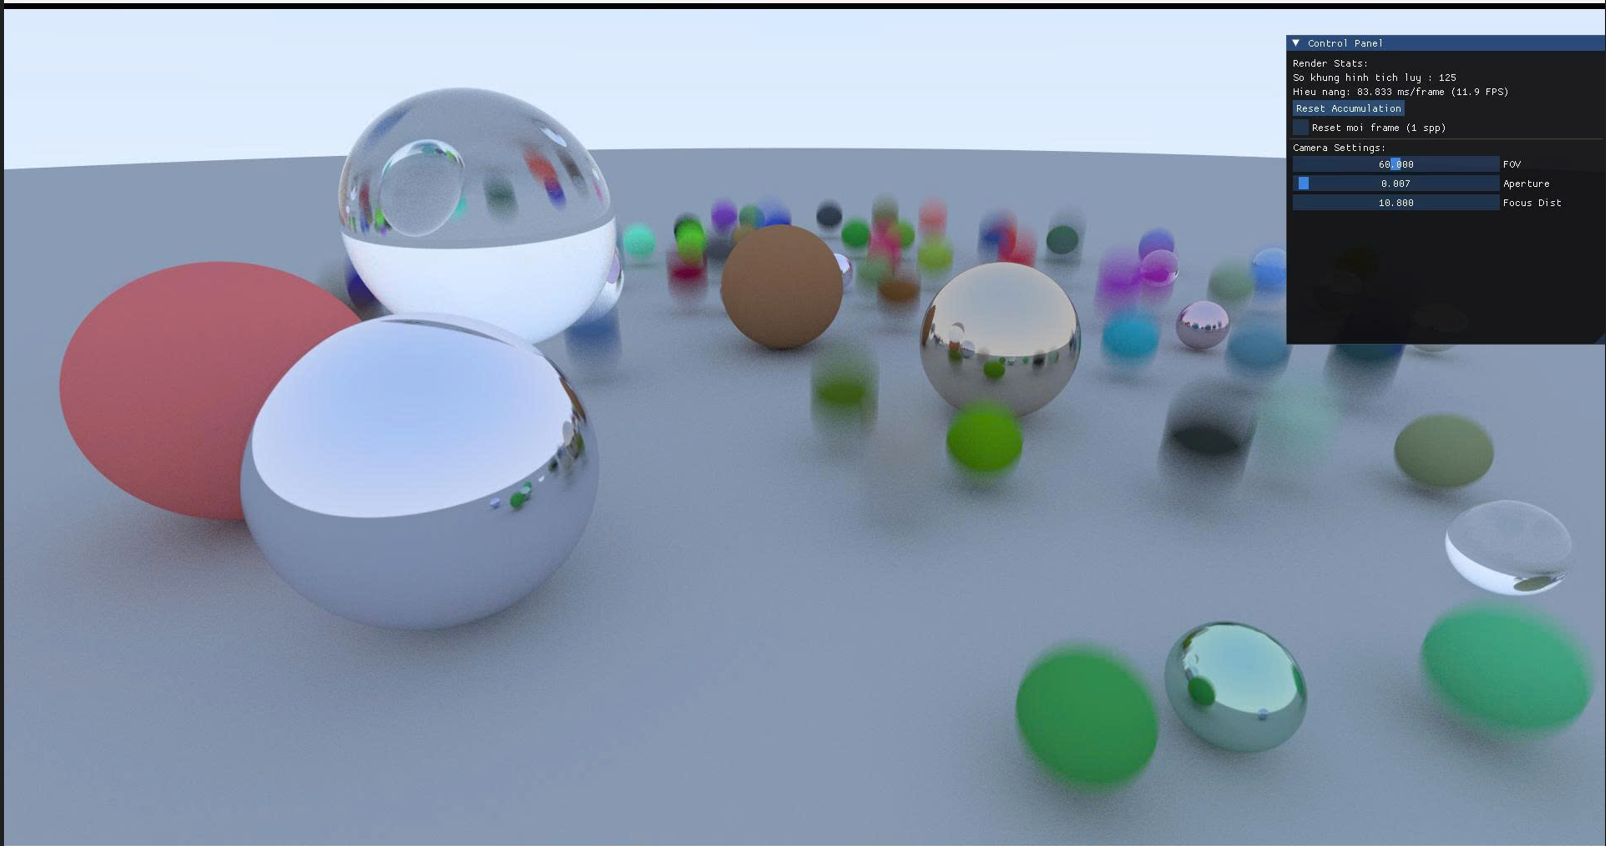
\includegraphics[width=\textwidth]{images/motion_blur.png}
  \caption{Nhòe chuyển động trên các khối cầu được gán vận tốc.}
  \label{fig:motion-blur}
\end{figure}

\section{Làm tối rìa ảnh (Vignetting)}
Hình~\ref{fig:vignette} minh họa hiệu ứng làm tối rìa ảnh áp dụng lên cảnh nhiều
vật liệu. Nguyên lý cốt lõi mà hiệu ứng này mô phỏng là định luật $\cos^4$ của
quang học ống kính: độ rọi tại một điểm trên phim lệch góc $\theta$ so với trục
quang giảm theo
\begin{equation}
\label{eq:cos4}
E(\theta) = E_0 \cos^4\theta,
\end{equation}
trong đó $E_0$ là độ rọi tại tâm ảnh. Số mũ 4 đến từ tích của bốn thừa số cosine:
khoảng cách từ thấu kính tới điểm ảnh xa hơn ở rìa đóng góp $\cos^2\theta$ theo
luật nghịch đảo bình phương, khẩu độ nhìn xiên nên diện tích chiếu giảm thêm
$\cos\theta$, và bề mặt phim nghiêng so với tia tới góp nốt $\cos\theta$. Vì
$\cos\theta$ giảm nhanh khi ra xa trục, độ sáng tụt mạnh ở bốn góc trong khi tâm
ảnh gần như không đổi. Hệ thống tái hiện quy luật này như một bước hậu xử lý điều
khiển bằng tham số Vignette: giá trị càng lớn thì vùng tối ở rìa càng rõ và mở
rộng vào trong, giúp hướng thị giác người xem vào chủ thể ở trung tâm.

\begin{figure}[H]
  \centering
  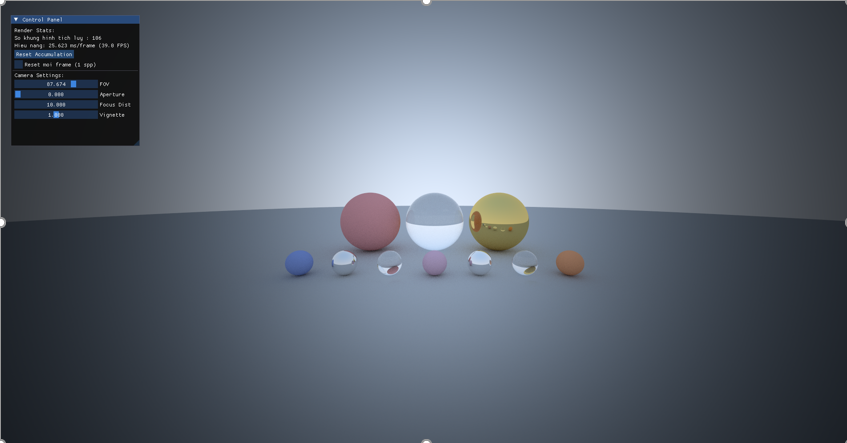
\includegraphics[width=\textwidth]{images/vignette.png}
  \caption{Hiệu ứng làm tối rìa ảnh (vignetting): độ sáng giảm dần từ tâm ra các góc khung hình.}
  \label{fig:vignette}
\end{figure}

\section{Nhận xét chung}
Qua các thử nghiệm trên, hệ thống tái tạo đầy đủ những hiệu ứng quang học mục
tiêu gồm phản xạ, khúc xạ, đổ bóng mềm, độ sâu trường ảnh và nhòe chuyển động,
với chất lượng hình ảnh hội tụ tốt sau vài trăm đến vài nghìn khung hình tích
lũy. Về hiệu năng, hệ thống duy trì tốc độ tương tác từ 10 đến 18 khung hình
trên giây với cảnh thưa, nhưng giảm rõ rệt khi mật độ vật thể tăng cao do chi phí
tìm giao điểm theo phương pháp duyệt tuyến tính. Kết quả này xác nhận tính đúng
đắn của hệ thống đồng thời chỉ ra nút thắt hiệu năng cần được giải quyết bằng cấu
trúc tăng tốc không gian, sẽ được bàn ở Chương~\ref{ch:ket-luan}.
